\section{Diagrama Entidad-Relación}
\subsection{Diagrama Entidad-Relación}
\begin{figure}[H]
   \begin{center}
   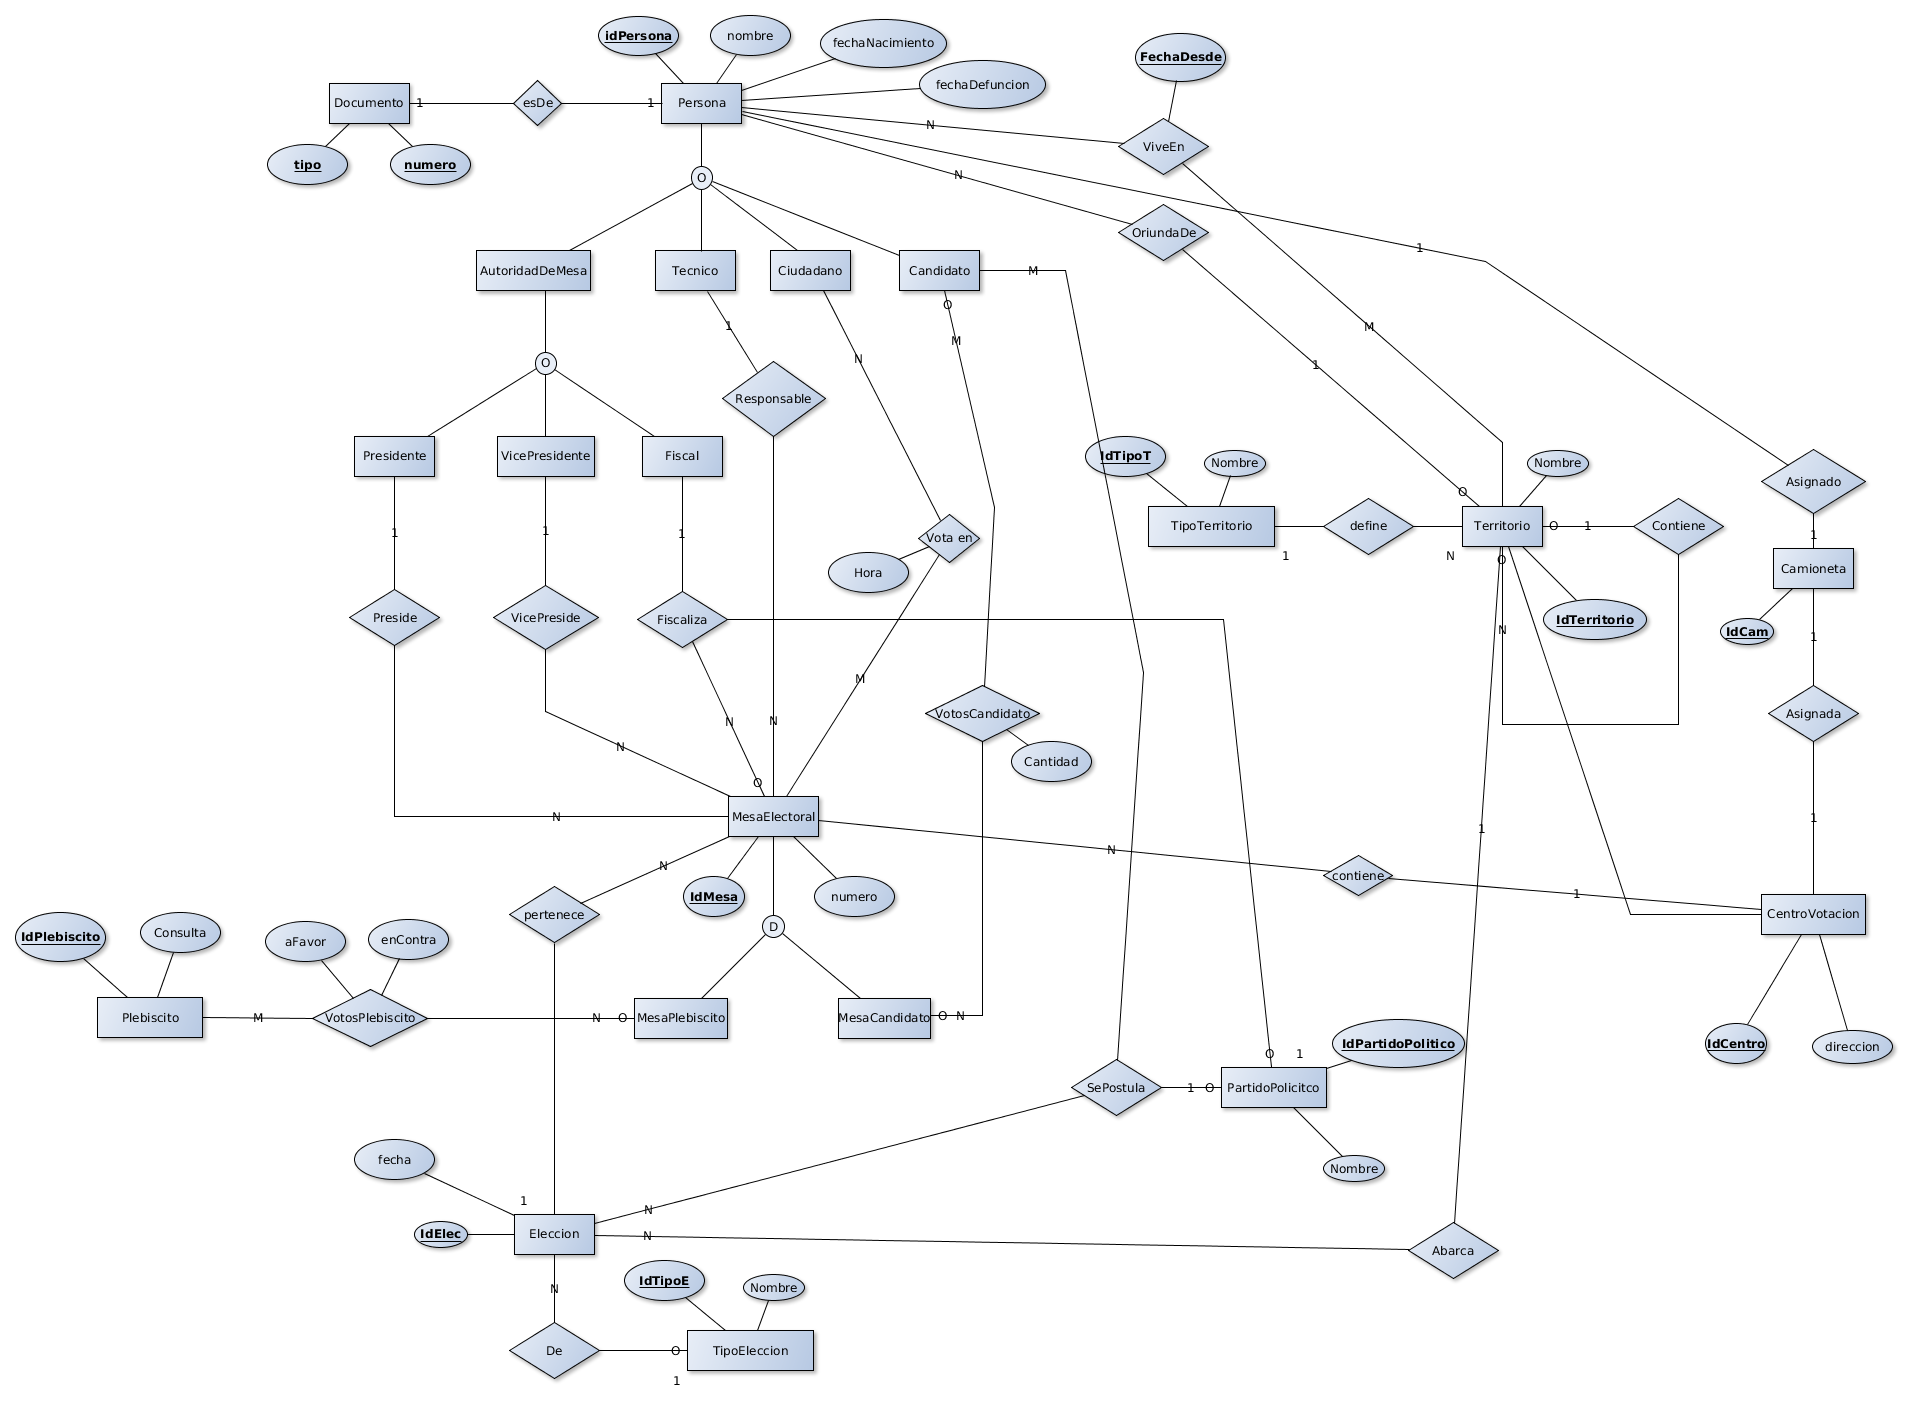
\includegraphics[angle=90,scale=0.32]{graphics/der.png}
   \caption{\textbf{Diagrama Entidad-Relación}}
   \label{fig:der}
   \end{center}
\end{figure}

\subsection{Restricciones Adicionales}

Sobre los atributos

* El número del DNI tiene que ser mayor a 0.
* El tipo del DNI tiene que ser alguno de los siguientes: DNI, CI, LE, LC.
* El atributo cantidad de la relación VotosCandidato tiene que ser mayor o igual a 0.
* El atributo nombre de TipoTerritorio debe ser alguno de los siguientes y no se pueden repetir:
  * País
  * Provincia
  * Localidad
  * Ciudad
* El número de la MesaElectoral tiene que ser mayor a 0.
* Los  atributos aFavor y enContra de la relación VotosPlebiscito  tienen que ser mayor o igual a 0.
* El atributo fechaNacimiento no puede ser posterior al atributo fechaDefunción.
* El atributo nombre de TipoEleccion debe ser alguno de los siguientes y no se pueden repetir:
*Presidencial
*Gobernador
*Intendente
*Plebiscito

Territorios sólo pueden contener a territorios más chicos.

* Un País sólo puede contener Provincias.
* Una Provincia sólo puede contener Localidades.
* Una Localidad sólo puede contener Ciudades.
* Una Ciudad no puede contener nada.

Sólo se puede ser oriundo de una ciudad.

Sólo los Territorios con TipoTerritorio de nombre "Ciudad" pueden participar de la relación OriundoDe.

Votar en las elecciones que corresponden según territorio.

Para que un Ciudadano pueda participar en VotosCandidato o VotosPlebiscito con la MesaElectoral correspondiente, ésta debe pertenecer a una Eleccion que abarque un Territorio el cual debe ser igual o contiene en algún nivel al Territorio en el cual el Ciudadano ViveEn en el momento de la elección[1].

[1] quien participa de ViveEn es Persona, no Ciudadano. Nos estamos refiriendo a la Persona correspondiente a dicho Ciudadano.

Presentarse como candidato para la elección de algún cargo.

Para que un Candidato pueda participar de SePostula con un PartidoPolítico en una Eleccion, el Territorio que esta última abarca debe ser igual o contener en algún nivel al Territorio en el cual el Candidato debe participar en ViveEn[2] con una fechaDesde mayor a los X años.

[2] Idem [1] pero para Candidato.

Solamente reciben votos los candidatos que se presentan a la elección.

Para que un Candidatos puede participar de VotosCandidato con MesaCandidato, debe participar en SePostula con la Elección a la cual la MesaElectoral pertenece.

Si el Partido Político tiene fiscales, tiene que postularse.

Para que PartidoPolítico participe de fiscaliza con una MesaElectoral, debe participar en sePostula con un Candidato en una Elección que contenga esa MesaElectoral.

Dentro de una Elección, los números de MesaElectoral no se pueden repetir.

Para cada elección, una Persona sólo puede ser Presidente, VicePresidente, Fiscal, Candidato o Técnico de manera disjunta.

Ciudadanos sólo pueden votarEn una única MesaElectoral por Elección.

No puede pasar que para una elección haya por lo menos una  MesasElectorales y por lo menos una MesaPlebiscito. 
No hay más votos que votantes

Para cada MesaCandidato, la sumatoria de cantidad en cada tupla de VotoCandidato debe ser menor igual a la cantidad de tuplas en la relación VotaEn entre MesaElectoral y Ciudadano.
Para cada MesaPlebiscito, la sumatoria de aFavor y enContra en cada tupla de VotoPlebiscito debe ser menor igual a la cantidad de tuplas en la relación VotaEn entre MesaElectoral y Ciudadano.

Mayor de 16 para votar

Para que una Persona sea Ciudadano tiene que tener más de 16 años.

Los muertos no votan

Para que un Ciudadano participe en VotaEn con una MesaElectoral, no debe tener fecha de defunción anterior a la fecha de la Elección correspondiente a esa Mesa.

No puede haber 2 o más  elecciones con misma fecha y mismo TipoEleccion para mismo Terrritorio. 

